\subsection{Injections Revisited}
\genHeader

Previously,we learned how to write handwritten code in an implementation file, then generate a \emph{partial class} to inject the corresponding code into the
metamodel.\footnote{See Part II, section 5} Now however, we'll generate and edit a partial class to automatically insert code into the corresponding Java file,
which will then be placed in the metamodel.

\begin{itemize}

\item[$\blacktriangleright$] Go to and open ``BoxImpl.java'' and, without editing anything in the file, generate its corresponding injection by
either right-clicking the file in the package explorer, or within the open editor window (Fig.~\ref{fig:createInjection}).

\vspace{0.5cm}

\begin{figure}[htbp]
    \centering
    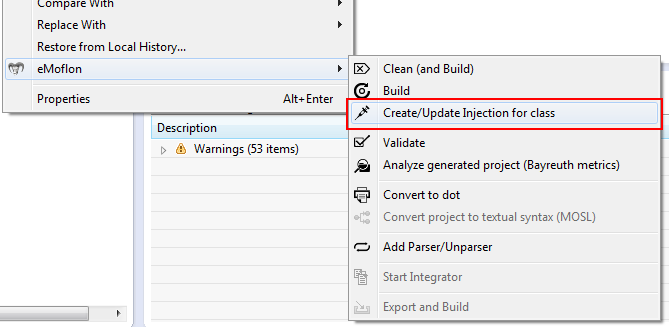
\includegraphics[width=0.9\textwidth]{eclipse_createBuildInjection}
    \caption{eMolfon context menu}
    \label{fig:createInjection}
\end{figure}

\clearpage

\item[$\blacktriangleright$] A lone file should now be placed in the \texttt{injection} folder.\footnote{Remember, you deleted \texttt{partition.impl} to start
the \texttt{removeCard} SDM} Open it and notice the partial class includes a signature for each method but (as expected), no implementation code
(Fig.~\ref{fig:injection_partialClassBox}).

\vspace{0.5cm}

\begin{figure}[htbp]
    \centering
    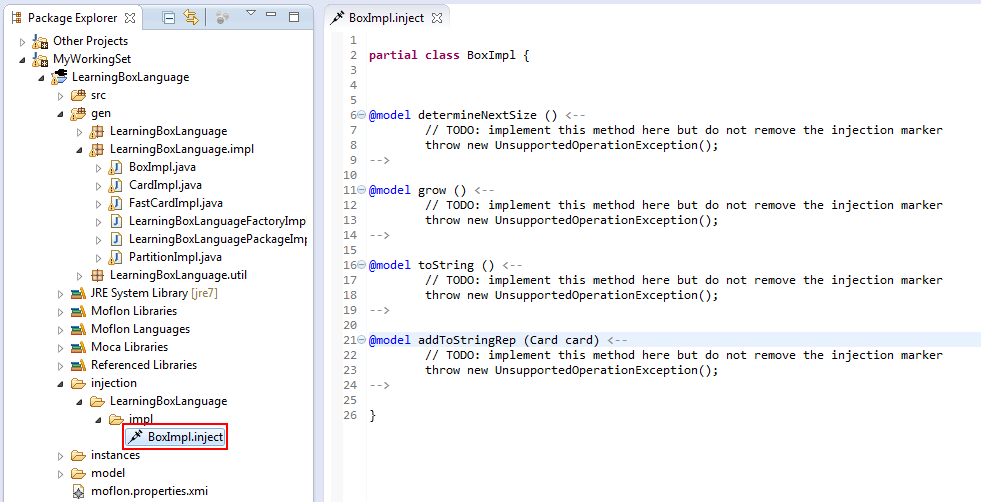
\includegraphics[width=\textwidth]{eclipse_injectionBoxImpl}
    \caption{Generated Injection file for \texttt{BoxImpl.java}}
    \label{fig:injection_partialClassBox}
\end{figure}

\vspace{0.5cm}

\item[$\blacktriangleright$] Complete \texttt{determineNextSize} as specified in Fig.~\ref{code:determine_inject_file}. To help avoid errors, this text can
be copied and pasted.

\vspace{0.5cm}

\item[$\blacktriangleright$] Finally, right-click the injection file, and rebuild your project by selecting ``eMoflon/Clean and Build.'' Go back to
\texttt{BoxImpl.java} and confirm that the helper methods have now been generated (Fig~\ref{fig:eclipse_updatedBoxImpl}).

\vspace{0.5cm}

\begin{figure}[h!]
        \centering
        \begin{lstlisting}[language=Java, keywordstyle={\bfseries\color{purple}}, backgroundcolor=\color{white}]
    @model determineNextSize () <--

            return getContainedPartition().size() * 10;
    -->

        \end{lstlisting}
        \caption{Developing \texttt{Box}'s \emph{partial class}}
        \label{code:determine_inject_file}
    \end{figure}
    \FloatBarrier

\newpage
\vspace*{1cm}

\begin{figure}[htbp]
    \centering
    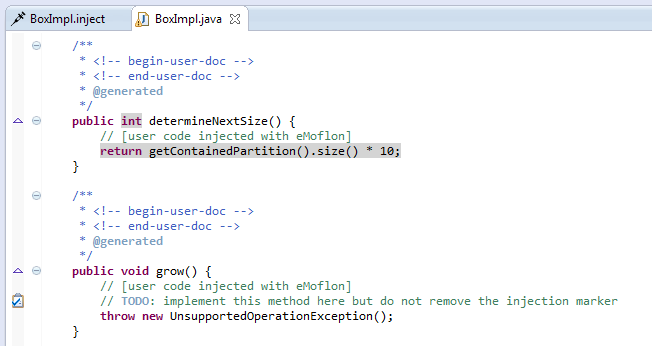
\includegraphics[width=\textwidth]{eclipse_updatedBoxImpl}
    \caption{Updated \texttt{BoxImpl.java} file}
    \label{fig:eclipse_updatedBoxImpl}
\end{figure}

\vspace{0.5cm}

\item[$\blacktriangleright$] Awesome - you're ready to start \texttt{grow}! For additional information on injections, check out Part IV: Miscellaneous. Be sure
to also review the work we completed with injections in Part II: Ecore.

\jumpDual{growBox vis}{growBox tex}

\end{itemize}